\chapter{Python简介}

\section{Python简介}

\subsection{编程简介}

程序(program)是为了让计算机执行某些操作或者解决问题而编写的一系列有序指令的集合。由于计算机只能够识别二进制数字0和1,因此需要使用特殊的编程语言来描述如何解决问题过程和方法。\\

算法(algorithm)是可完成特定任务的一系列步骤,算法的计算过程定义明确,通过一些值作为输入并产生一些值作为输出。\\

流程图(flow chart)是算法的一种图形化表示方式,使用一组预定义的符号来说明如何执行特定任务。

\begin{itemize}
	\item 圆角矩形:开始和结束
	\item 矩形:数据处理
	\item 平行四边形:输入/输出
	\item 菱形:分支判断条件
	\item 流程线:步骤
\end{itemize}

\vspace{0.5cm}

\begin{figure}
	\centering
	\begin{tikzpicture}[node distance=2cm]
		\node (start) [startend] {Start};
		\node (init)   [io, below of=start] {$ i = 0 $, $ sum = 0 $};
		\node (decision)  [decision, below of=init] {$ i \le 100 $?};
		\node (accumulation) [process, below of=decision] {$ sum = sum + i $};
		\node (update) [process, below of=accumulation] {$ i = i + 1 $};
		\node (output) [io, right of=decision, xshift=2.5cm] {print $ sum $};
		\node (end) [startend, below of=update] {End};

		\draw [arrow] (start) -- (init);
		\draw [arrow] (init) -- (decision);
		\draw [arrow] (decision) -- node[anchor=east] {yes } (accumulation);
		\draw [arrow] (accumulation) -- (update);
		\draw [arrow] (update) -- (-3,-8) -- (-3,-4) -- (decision);
		\draw [arrow] (decision) -- node[anchor=south] {no} (output);
		\draw [arrow] (output) |- (end);
	\end{tikzpicture}
	\caption{计算$ \sum_{i=1}^{100} i $的流程图}
\end{figure}

\subsection{Python简介}

在当今的环境下Python是一个热门语言,在全世界的范围内,许多大学都开始使用Python作为基础语言的教程,同时在数据分析领域以及人工智能领域也取得了显著的成绩。\\

Python最大的特点就是简单。同样的一个功能,使用C语言实现需要20行代码,Java需要10行代码,Python的实现只需要4行代码,它从整体的代码量而言是非常简洁的。

\begin{itemize}
	\item Python具有很强的可读性,比其他语言更有特色语法结构。
	\item Python是解释型语言,这意味着开发过程中没有了编译环节。
	\item Python是交互式语言,这意味着可以在提示符后直接执行代码。
	\item Python是面向对象语言,这意味着支持面向对象的风格和代码封装。
\end{itemize}

虽然Python提供有交互式的命令模式,但是在很多的情况下,对于程序的编写往往是将其定义在源文件之中,在Python里面所有的源文件的后缀名称必须是.py。

\begin{figure}[H]
	\centering
	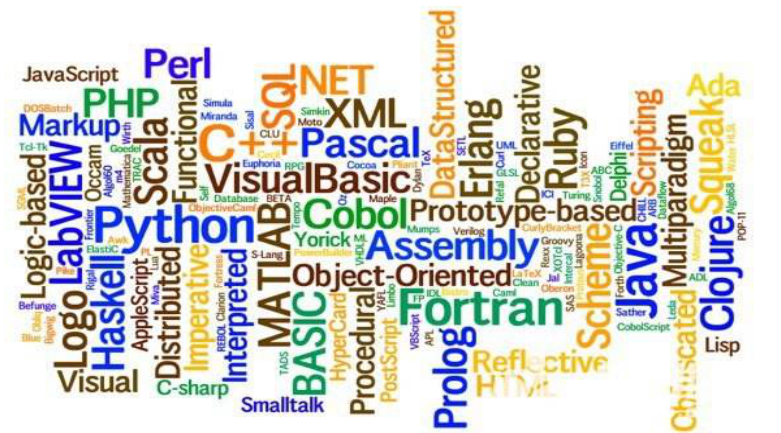
\includegraphics[scale=0.9]{img/C1/1-1/1.png}
	\caption{常见编程语言}
\end{figure}

\vspace{0.5cm}

\subsection{Hello World!}

输出的时候使用print()函数,函数就是一个完成特定功能的代码组织结构。\\

\mybox{Hello World!}

\begin{lstlisting}[language=Python]
print("Hello World!")
\end{lstlisting}

\begin{tcolorbox}
	\mybox{运行结果}
	\begin{verbatim}
Hello World!
	\end{verbatim}
\end{tcolorbox}

\newpage

\section{注释}

\subsection{注释(Comment)}

在进行项目的开发过程中,不可能说一个项目编写完成一次后就在也不进行修改了。所以很多情况下,为了方便下一次的修改,会在一些关键性的代码上进行一些注释信息的定义,开发者根据这些注释的文字信息就可能直到这段代码的主要作用,方便代码的维护。\\

Python里面的注释分为两类:

\begin{enumerate}
	\item 单行注释:将一行内【\#】之后的内容视为注释。
	\item 多行注释:三引号中间的内容视为注释。
\end{enumerate}

\vspace{0.5cm}

\mybox{注释}

\begin{lstlisting}[language=Python]
"""
这是一条
多行注释
"""
print("Hello World!")		# 输出Hello World!
\end{lstlisting}

\begin{tcolorbox}
	\mybox{运行结果}
	\begin{verbatim}
Hello World!
	\end{verbatim}
\end{tcolorbox}

\newpage

\section{标识符}

\subsection{标识符(Identifier)}

标识符的第一个字符必须是字母表中字母或下划线【\_】,标识符的其它部分由字母、数字和下划线组成,标识符对大小写敏感。标识符不可以使用保留字或关键字。标识符应该准确、顾名思义,不要使用汉语拼音。\\

关键字(key word)也称保留字,关键字是编程语言内置的一些名称,具有特殊的用处和意义。保留字不能用作于标识符名称。Python的标准库提供了一个keyword模块,可以输出当前版本的所有关键字。\\

\mybox{关键字}

\begin{lstlisting}[language=Python]
import keyword
print(keyword.kwlist)
\end{lstlisting}

\begin{table}[H]
	\centering
	\setlength{\tabcolsep}{5mm}{
		\begin{tabular}{|c|c|c|c|c|}
			\hline
			False  & None  & True   & and      & as      \\
			\hline
			assert & break & class  & continue & def     \\
			\hline
			del    & elif  & else   & except   & finally \\
			\hline
			for    & from  & global & if       & import  \\
			\hline
			in     & is    & lambda & nonlocal & not     \\
			\hline
			or     & pass  & raise  & return   & try     \\
			\hline
			while  & with  & yield  &          &         \\
			\hline
		\end{tabular}
	}
	\caption{关键字}
\end{table}

\vspace{0.5cm}

\subsection{变量(Variable)}

在程序之中所谓的变量指的是可以被改变的内容,而常量指的是绝对不会被改变的内容。Python语言最大的特点是变量都是可以被直接定义的,不需要那些复杂的数据类型的声明,直接使用变量名称即可。\\

所有的变量实际上都会占据内存空间,当一些变量不再使用的时候,可以使用del关键字对内存空间进行删除。变量一旦被删除了,那么后续的代码部分将无法继续使用它。\\

\mybox{变量}

\begin{lstlisting}[language=Python]
num = 10
print(num)
del num
print(num)
\end{lstlisting}

\begin{tcolorbox}
	\mybox{运行结果}
	\begin{verbatim}
10
NameError: name 'a' is not defined
	\end{verbatim}
\end{tcolorbox}

\newpage

\section{数据类型}

\subsection{数据类型}

Python中的变量不需要声明,但是每个变量在使用前都必须赋值,变量赋值以后该变量才会被创建。在Python中变量没有类型,我们所说的“类型”是变量所指的内存中对象的类型。使用type()函数可以获取变量的数据类型。\\

在Python中使用等号【=】用来给变量赋值,赋值运算符左边是一个变量名,赋值运算符右边是存储在变量中的值。\\

布尔是19世纪一位英国数学家的名字,在开发之中布尔主要用于程序的逻辑分支处理,数值包括True和False。\\

按照各个传统编程语言的做法来讲,整数 / 整数 = 整数,但是Python认为这个结果应该包含有小数(整数的结果变为浮点数类型)。\\

\mybox{数据类型}

\begin{lstlisting}[language=Python]
num = 123		# 整型
PI = 3.1415		# 浮点型
s = "hello"		# 字符串
flag = True		# 布尔

print(num)
print(PI)
print(s)
print(flag)

print(type(num))
print(type(PI))
print(type(s))
print(type(flag))

print(10 / 4)
print(type(10 / 4))
\end{lstlisting}

\begin{tcolorbox}
	\mybox{运行结果}
	\begin{verbatim}
123
3.1415
hello
True
<class 'int'>
<class 'float'>
<class 'str'>
<class 'bool'>
2.5
<class 'float'>
	\end{verbatim}
\end{tcolorbox}

\vspace{0.5cm}

\subsection{字符串(String)}

字符串是开发中最为重要的概念,一个编程语言是否好用,很大程度上也是取决于是否提供有字符串类型。Python中可以直接使用引号(单引号或双引号)进行字符串的定义。Python并没有字符的概念,所以对于引号表示的含义是相同的。\\

使用【+】运算符可以进行字符串的连接处理。\\

\mybox{字符串连接}

\begin{lstlisting}[language=Python]
str = "Hello" + "World"
str += "!"
print(str)
\end{lstlisting}

\begin{tcolorbox}
	\mybox{运行结果}
	\begin{verbatim}
HelloWorld!
	\end{verbatim}
\end{tcolorbox}

\vspace{0.5cm}

\subsection{转义字符}

在一个字符串描述的过程中,有可能会有一些特殊字符的信息。

\begin{table}[H]
	\centering
	\setlength{\tabcolsep}{5mm}{
		\begin{tabular}{|c|c|}
			\hline
			\textbf{转义字符}      & \textbf{描述}                        \\
			\hline
			\lstinline|\\| & 表示一个反斜杠\lstinline|\| \\
			\hline
			\lstinline|\'| & 表示一个单引号\lstinline|'| \\
			\hline
			\lstinline|\"| & 表示一个双引号\lstinline|"| \\
			\hline
			\lstinline|\n| & 换行                                 \\
			\hline
			\lstinline|\t| & 横向制表符                           \\
			\hline
		\end{tabular}
	}
	\caption{转义字符}
\end{table}

\mybox{转义字符}

\begin{lstlisting}[language=Python]
print("全球最大同性交友网站\n\"https://github.com\"")
\end{lstlisting}

\begin{tcolorbox}
	\mybox{运行结果}
	\begin{verbatim}
全球最大同性交友网站
"https://github.com"
	\end{verbatim}
\end{tcolorbox}

\newpage

\section{数据输入}

\subsection{input()}

input()用于接受键盘输入。在所有编程语言里面,输入数据的类型是字符串类型。\\

\mybox{数据输入}

\begin{lstlisting}[language=Python]
data = input("输入数据:")
print(data)
print(type(data))
\end{lstlisting}

\begin{tcolorbox}
	\mybox{运行结果}
	\begin{verbatim}
输入数据:123
123
<class 'str'>
	\end{verbatim}
\end{tcolorbox}

\vspace{0.5cm}

\subsection{转换函数}

很多时候可能需要的是各种类型,例如:整数、浮点数、布尔型,或者将其它类型变为字符串型。如果字符串不是由数字所组成,那么程序的执行就会产生异常。

\begin{table}[H]
	\centering
	\setlength{\tabcolsep}{5mm}{
		\begin{tabular}{|c|l|}
			\hline
			\textbf{函数} & \textbf{功能}              \\
			\hline
			int(数据)     & 将指定数据转为整型数据     \\
			\hline
			float(数据)   & 将指定数据转为浮点型数据   \\
			\hline
			bool(数据)    & 将指定数据转为布尔型数据   \\
			\hline
			str(数据)     & 将指定数据转为字符串型数据 \\
			\hline
		\end{tabular}
	}
	\caption{转换函数}
\end{table}

\mybox{加法计算(Bug版本)}

\begin{lstlisting}[language=Python]
num1 = float(input("输入第一个数字:"))
num2 = float(input("输入第二个数字:"))
result = num1 + num2
print(num1 + "+" + num2 + "=" + result)
\end{lstlisting}

\begin{tcolorbox}
	\mybox{运行结果}
	\begin{verbatim}
输入第一个数字:11.1
输入第二个数字:22.2
TypeError: unsupported operand type(s) for +: 'float' and 'str'
	\end{verbatim}
\end{tcolorbox}

\vspace{0.5cm}

\mybox{加法计算(正确版本)}

\begin{lstlisting}[language=Python]
num1 = float(input("输入第一个数字:"))
num2 = float(input("输入第二个数字:"))
result = num1 + num2
print(str(num1) + "+" + str(num2) + "=" + str(result))
\end{lstlisting}

\begin{tcolorbox}
	\mybox{运行结果}
	\begin{verbatim}
输入第一个数字:11.1
输入第二个数字:22.2
11.1+22.2=33.3
	\end{verbatim}
\end{tcolorbox}

\newpage

\section{格式化输出}

\subsection{格式化输出}

为了解决数据的输出问题,Python提供有格式化的输出操作。

\begin{table}[H]
	\centering
	\setlength{\tabcolsep}{5mm}{
		\begin{tabular}{|c|l|}
			\hline
			\textbf{标记} & \textbf{功能}                      \\
			\hline
			\%c           & 格式化字符                         \\
			\hline
			\%s           & 格式化字符串                       \\
			\hline
			\%d           & 格式化整型                         \\
			\hline
			\%f           & 格式化浮点型,可以设置保留精度     \\
			\hline
			\%e           & 科学计数法,使用小写字母e          \\
			\hline
			\%E           & 科学计数法,使用大写字母e          \\
			\hline
			\%g           & \%f和\%e的简写                     \\
			\hline
			\%G           & \%f和\%E的简写                     \\
			\hline
			\%u           & 格式化无符号整型                   \\
			\hline
			\%o           & 格式化无符号八进制数               \\
			\hline
			\%x           & 格式化无符号十六进制数             \\
			\hline
			\%X           & 格式化无符号十六进制数(大写字母) \\
			\hline
		\end{tabular}
	}
	\caption{格式化输出}
\end{table}

\mybox{格式化字符串}

\begin{lstlisting}[language=Python]
name = "小灰"
age = 16
height = 175.6

print("姓名:%s,年龄:%d,身高:%.2f" % (name, age, height))
\end{lstlisting}

\begin{tcolorbox}
	\mybox{运行结果}
	\begin{verbatim}
姓名:小灰,年龄:16,身高:175.60
	\end{verbatim}
\end{tcolorbox}

\vspace{0.5cm}

\subsection{分隔符}

在默认情况下,使用print()输出数据时,都会使用换行作为分隔符号。如果不希望使用换行,则可以追加一个end参数。\\

\mybox{分隔符}

\begin{lstlisting}[language=Python]
sequence = "1 2 4 8 16 32 64"
print("序列:", end='')
print(sequence, end='...')
\end{lstlisting}

\begin{tcolorbox}
	\mybox{运行结果}
	\begin{verbatim}
序列:1 2 4 8 16 32 64...
	\end{verbatim}
\end{tcolorbox}

\newpage

\section{运算符}

\subsection{算术运算符}

\begin{table}[H]
	\centering
	\setlength{\tabcolsep}{5mm}{
		\begin{tabular}{|c|l|}
			\hline
			\textbf{运算符} & \textbf{功能}                              \\
			\hline
			+               & 两个数相加                                 \\
			\hline
			-               & 得到负数或一个数减去另一个数               \\
			\hline
			*               & 两个数相乘或是返回一个被重复若干次的字符串 \\
			\hline
			/               & 两数相除                                   \\
			\hline
			\%              & 返回除法的余数                             \\
			\hline
			**              & 幂                                         \\
			\hline
			//              & 整除(向下取整)                           \\
			\hline
		\end{tabular}
	}
	\caption{算术运算符}
\end{table}

\mybox{计算圆的面积}

\begin{lstlisting}[language=Python]
PI = 3.14159
r = float(input("输入半径:"))
area = PI * r ** 2
print("面积 = %.2f" % area)
\end{lstlisting}

\begin{tcolorbox}
	\mybox{运行结果}
	\begin{verbatim}
输入半径:5
面积 = 78.54
	\end{verbatim}
\end{tcolorbox}

\vspace{0.5cm}

\mybox{逆序三位数}

\begin{lstlisting}[language=Python]
num = int(input("输入一个正三位数:"))
a = num // 100
b = num // 10 % 10
c = num % 10
print("逆序:%d" % (c*100 + b*10 + a))
\end{lstlisting}

\begin{tcolorbox}
	\mybox{运行结果}
	\begin{verbatim}
输入一个正三位数:520
逆序:25
	\end{verbatim}
\end{tcolorbox}

\vspace{0.5cm}

\subsection{复合赋值运算符}

\begin{table}[H]
	\centering
	\setlength{\tabcolsep}{5mm}{
		\begin{tabular}{|c|l|}
			\hline
			\textbf{运算符} & \textbf{功能}           \\
			\hline
			+=              & a += b等价于a = a + b   \\
			\hline
			-=              & a -= b等价于a = a - b   \\
			\hline
			*=              & a *= b等价于a = a * b   \\
			\hline
			/=              & a /= b等价于a = a / b   \\
			\hline
			\%=             & a \%= b等价于a = a \% b \\
			\hline
			**=             & a **= b等价于a = a ** b \\
			\hline
			//=             & a //= b等价于a = a // b \\
			\hline
		\end{tabular}
	}
	\caption{复合赋值运算符}
\end{table}

\vspace{0.5cm}

\subsection{比较运算符}

\begin{table}[H]
	\centering
	\setlength{\tabcolsep}{5mm}{
		\begin{tabular}{|c|c|}
			\hline
			\textbf{运算符} & \textbf{功能} \\
			\hline
			==              & 等于          \\
			\hline
			!=              & 不等于        \\
			\hline
			>               & 大于          \\
			\hline
			<               & 小于          \\
			\hline
			>=              & 大于等于      \\
			\hline
			<=              & 小于等于      \\
			\hline
		\end{tabular}
	}
	\caption{比较运算符}
\end{table}

\newpage